\documentclass{crypto-exercise}
\usepackage{amsthm}
\usepackage{amsthm}
\author[Fiat-Shamir]{Sven Laur}
\contributor[Initial solution scheme]{Filipp Ivanov}
\contributor[Full solution]{Sven Laur}
\editor{Sven Laur}
\tags{statistical indistinguishability, distributions, zero-knowledge, quadratic non-residuosity proof}

\renewcommand{\ADVIND}[2]{\ADV^{\mathsf{ind}}_{#1}(#2)}
\newcommand{\REWRITE}{\qquad\scalebox{1.5}{$\rightsquigarrow$}\qquad}
\newcommand{\ISQNR}{\mathsf{IsQnr}}
\newcommand{\SFAIL}{\mathsf{SimFail}}

\begin{document}


\begin{exercise}{Standard simulator for the QNR-ZK protocol}
Let $n$ be a composite number with a factorisation $n=pq$ known to the prover $\PPP$. Let $v\in\ZZ_n^*$ be a number for which the prover wants to prove that it is quadratic non-residue. Show that the the following zero-knowledge protocol    
\begin{center}
\begin{tabular}{lllcl}
	&$\PPP$ &&   $\VVV$\\
	&&&& $b\getsu\set{0,1},\ $\\
    &&$\xleftarrow{\makebox[4cm]{$c=r^2v^b$}}$ 
	&& $r\getsu\ZZ_n^*$ \\
	\\
	\phantom{$\xleftarrow {\makebox[0cm]{$\beta$}}$} 
	&&$\xleftarrow {\makebox[4cm]{$\alpha$}}$ 
	&& $\alpha\gets\PPP_{\mathrm{POK}}$\\
	$\beta\gets\BBB$
	&&$\xrightarrow{\makebox[4cm]{{$\beta$}}}$\\
	$\VERIFY(\alpha,\beta,\gamma)\iseq 1$
	\phantom{$\xleftarrow {\makebox[0cm]{$\beta$}}$} 
	&&$\xleftarrow {\makebox[4cm]{\smash{$\gamma$}}}$ 
	&& $\gamma\gets\PPP_{\mathrm{POK}}(\beta)$\\
	\\
	$\overline{b}\gets\ISQNR_{p,q}(c)$
	&&$\xrightarrow{\makebox[4cm]{$\overline{b}$}}$
	&& $\overline{b}\iseq b$
	\\
\end{tabular}
\end{center}   
where the verifier $\VVV$ uses sigma protocol $\POK[\exists r, \beta: c = r^2v^b]$ to prove the knowledge of $b$ and $r$ is simulatable. More precisely, let $\KEXTR^{\VVV_*}$ standard knowledge extractor for the protocol $\POK[\exists r, \beta: c = r^2v^b]$. Then show that the following simulator construction
\begin{align*}
\begin{fblock}{\VVV_\circ(\phi)}
 & \omega\gets\Omega\\
 & c\gets\VVV_*(\phi;\omega)\\
 & (b_*,r_*)\gets\KEXTR^{\VVV_*}(\phi;\omega)\\
 & \alpha\gets\VVV_*\\
 & \beta\getsu\BBB\\
 & \gamma\gets\VVV_*(\beta)\\
 & \IF \VERIFY(\alpha,\beta,\gamma)=0\ \THEN \RETURN \VVV_*(\bot)\\ 
 & \IF \beta_*\neq \bot \ \THEN \RETURN \VVV_*(b_*)\\
 & \ELSE \RETURN \bot
\end{fblock}
\end{align*}   
can create an output distribution $\psi_\circ$ that is statistically $\varepsilon_\circ$-distant from the output distribution of malicious verifier $\VVV_*$ that interacts with the honest prover. Also, estimate how the running-time of the simulator depends on the desired statistical distance $\varepsilon_\circ$.
\end{exercise}
\begin{solution}
For the analysis, let us contrast the simulation with the real-world execution. For that we  observe when the execution of a simulator diverges form the real-world interaction between $\VVV(\phi)$ and  $\PPP$ provided that the randomness of the verifier $\omega\gets\Omega$ is same. Again, it is instructive to see the event trees first, see Figure~\ref{fig:event-trees}. 
On the left you see the execution corresponding to the simulation. On the right you see the real protocol execution augmented with the run of the knowledge extractor. Here, the protocol run does not use knowledge-extraction for anything, it just provides the same split of events.   
 
First, observe that the simulation and real-world execution are identical till the last verification step of $\POK[\exists r, \beta: c = r^2v^b]$, since all messages are created exactly the same way in both runs. If the verification fails, then the verifier gets the same input in both executions. Hence, we must consider the remaining case. Clearly, executions diverge when the knowledge-extraction fails. In the remaining case, $\VVV$ receives $\overline{b}$ in the real execution and $b_*$ in the simulation. Hence, we must show that $\overline{b}=b_*$. 

The latter reveals a small but important detail in the knowledge proof. Namely, it is straightforward to see that any invertible element $c$ one has only two possible decompositions: $c=r^2v^b$ and $c=(-r)^2v^b$ if the Jacobi symbols of $v$ and $c$ match.
Thus, $b_*$ must be equal to $\overline{b}$. However, if the Jacobi symbols of $v$ and $c$ are not both ones, the existence of the decomposition is not guaranteed and we cannot conclude that $b_*=\overline{b}$. Fortunaltely, in the first step of the proof of knowledge the verifying party checks that $v$ and $c$ are in the suitable form and the same is done in the knowledge extractor. Hence, the claim $b_*=\overline{b}$ holds. 

\begin{figure}[!h]
   \centering
   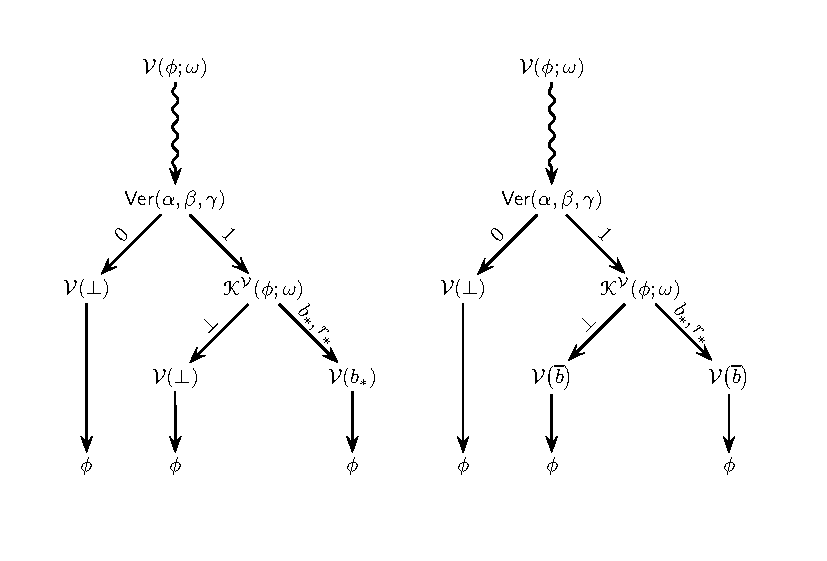
\includegraphics[scale=0.85]{figures/1102-event-tree-i}
   \caption{Event trees for the protocol simulation and for real protocol execution.}
   \label{fig:event-trees}
\end{figure}

These observations combined with the the following lemma allow us to estimate the statistical distance by computing the probability of the event that verification succeeds while knowledge error fails. 
 
\vspace*{2ex}
\noindent\textbf{Lemma.}
\begin{it}
If two strategies start to diverge only after the event $\mathsf{div}$ and and are identical before that the the statistical distance between the output distributions is at most $\pr{\mathsf{div}}$.  
\end{it} 
\begin{proof}
Let $\SSS_1$ and $\SSS_2$ be the strategies in question and $\psi_1$ and $\psi_2$ corresponding output distributions. Then by the definition
\begin{align*}
\SD(\psi_1,\psi_2)&=\frac{1}{2}\cdot \sum_{\phi}\abs{\pr{\phi_1\gets\SSS_1: \phi_1=\phi}-\pr{\phi_2\gets\SSS_2: \phi_2=\phi }}\\
&=\frac{1}{2}\cdot \sum_{\phi}\abs{\pr{\phi_1\gets\SSS_1: \phi_1=\phi\wedge \mathsf{div}}-\pr{\phi_2\gets\SSS_2: \phi_2=\phi\wedge \mathsf{div}}}\\
&\quad+\frac{1}{2}\cdot \sum_{\phi}\abs{\pr{\phi_1\gets\SSS_1: \phi_1=\phi\wedge \neg\mathsf{div}}-\pr{\phi_2\gets\SSS_2: \phi_2=\phi\wedge \neg\mathsf{div}}}\\
&=\frac{1}{2}\cdot \sum_{\phi}\abs{\pr{\phi_1\gets\SSS_1: \phi_1=\phi\wedge \mathsf{div}}-\pr{\phi_2\gets\SSS_2: \phi_2=\phi\wedge \mathsf{div}}}\\
&\leq \frac{1}{2}\cdot \sum_{\phi}\pr{\phi_1\gets\SSS_1: \phi_1=\phi\wedge \mathsf{div}}+ \frac{1}{2}\cdot \sum_{\phi}\pr{\phi_2\gets\SSS_2: \phi_2=\phi\wedge \mathsf{div}}\\
&\leq \frac{1}{2}\cdot \pr{\phi_1\gets\SSS_1: \mathsf{div}}+ \frac{1}{2}\cdot \pr{\phi_2\gets\SSS_2: \mathsf{div}}\leq \pr{\mathsf{div}}\enspace
\end{align*} 
Note that by the construction the event $\mathsf{div}$ has the same probability for both strategies since up to this procedure both systems are identical and thus $\pr{\mathsf{div}}$ is well defined.
\end{proof}

For brevity, let  $\SFAIL$ denote the event that verification succeeds while knowledge error fails. As the probability of this event  may depend on the randomness $\omega$, we must configure the knowledge extractor so that the corresponding probability is negligible on average over all possible $\omega\in\Omega$ . First  all all the failure probability can be high for fixed $\omega$ only if verification succeeds and knowledge error fails with non-negligible probability. Intuitively, achieving such a bad case is a careful balancing act, since higher success probability on verification also increases the success of $\KEXTR^{\VVV}(\phi;\omega)$. Figure~\ref{fig:simulation-failure} illustrates the corresponding behaviour.

\begin{figure}[!h]
   \centering
   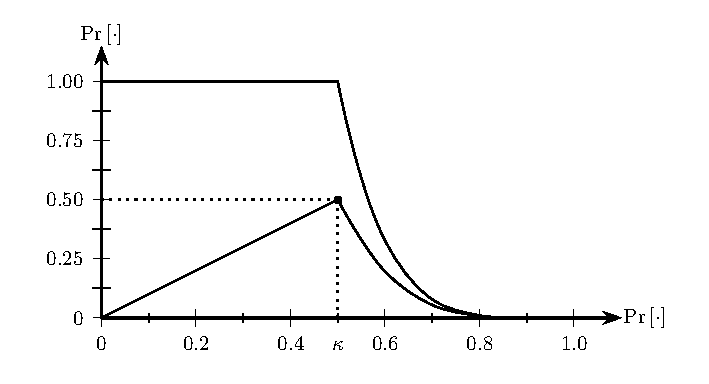
\includegraphics[scale=0.85]{figures/1102-simulation-failure-i}
   \caption{Knowledge-extraction failure as function of verification success. The $x$-axis corresponds to the verification success and $y$-axis corresponds to the failure probability. The upper graph corresponds to the knowledge extraction failure and the lower graph corresponds to the simulation failure. The plot is drawn for the knowledge extractor that does $10$ probes. In reasonable simulation construections $\ell\gg 10$ and the drop after the $\frac{1}{2}$ is extremely sharp and the optimum does not change for fixed running-time simulators.}
   \label{fig:simulation-failure}
\end{figure}

Figure~\ref{fig:simulation-failure} clearly shows that the worst configuration is such that $\pr{\VERIFY(\alpha,\beta,\gamma)=1}=\frac{1}{2}$ for which the simulation failure $\SFAIL$ occurs with probability $\frac{1}{2}$. The latter holds for fixed randomness $\omega\in\Omega$. Thus, the worst adversarial configuration for the simulation is such that it will succeed the proof of knowledge with probability $\frac{1}{2}$. As a result, 
\begin{align*}
\pr{\SFAIL}=\sum_{\omega\in\Omega}\pr{\omega}\cdot\pr{\SFAIL|\omega}=\frac{1}{2}
\end{align*}  
and the lemma provides a poor bound on the statistical distance:
\begin{align*}
\SD(\psi_1,\psi_2)\leq \pr{\SFAIL}=\frac{1}{2}\enspace.
\end{align*}  
The bound is sharp. If the malicious verifier chooses a random challenge or a challenges obtained prior to the beginning of the protocol. Then the verifier can cheat in the proof of knowledge by first guessing $\beta$ and then simulating the triple using the canonical simulator $\SSS$. As a result, the verifier will learn the quadratic residuosity of $c$ with probability $\frac{1}{2}$. Under the standard assumptions detecting quadratic residuosity is intractable problem and thus no efficient simulator that achieves $\SD(\psi_1,\psi_2)\ll \frac{1}{2}$ can exist.      

\paragraph{Naive protocol upgrade.}
The large discrepancy in the simulation is doused by the high knowledge error. The simplest solution is to repeat the proof-of-knowledge protocol $k$ times. As a result, the knowledge-error $\kappa$ decreases form $\frac{1}{2}$ to $2^{-k}$. However, the lower knowledge error alone does not guarantee a small simulation failure, the the knowledge-extraction must be successful enough when $\varepsilon>\kappa$. To understand the logic behind the simulation of multi-stage proof-knowledge, it is instructive to look at Figure~\ref{fig:proof-event-tree}.  

\begin{figure}[!h]
   \centering
   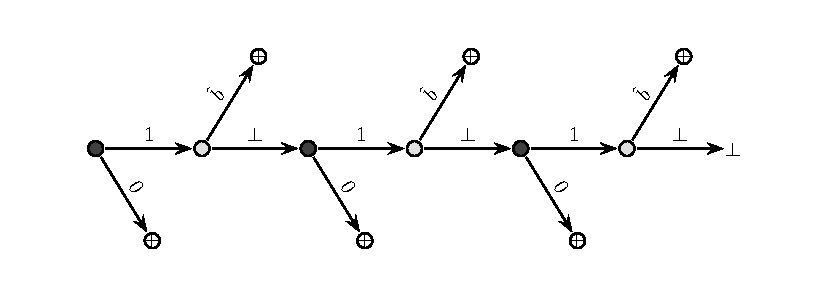
\includegraphics[scale=0.85]{figures/1102-event-tree-ii}
   \caption{Combined simulation and knowledge extraction in case of a multi-stage proof of knowledge. Black dots represent verification stages doting the simulation. Grey dots represent knowledge-extraction phases following successful verification stages. Dots with crosses denote states where perfect simulation if achievable either because a verification stage failed or because a knowledge-extraction yielded the desired witness. In these cases, perfect simulation of the protocol becomes trivial.}
   \label{fig:proof-event-tree}
\end{figure}

By the construction the events on each stage are independent form the previous stages. The
stage fails if the verification succeeds but knowledge extraction fails. This stage failure depends on the adversaries behaviour. However, as the stage failure is identical to the simulation failure of  the knowledge proof, it is easy to guarantee that the stage failure probability is below $\frac{1}{2}$. Thus, the statistical distance between verifiers outputs in the simulation and real protocol execution is well bounded:
\begin{align*}
\SD(\psi_1,\psi_2)\leq \pr{\SFAIL}\cdot\ldots\cdot\pr{\SFAIL} \leq 2^{-k}\enspace.
\end{align*}        

This bound leads to an interesting observation about knowledge-extraction stategy. The knowledge extraction does not have to be very successful to get a simulation profile that is bounded above by $\frac{1}{2}$. By simple analysis we can show that the failure probability of a standard knowledge extractor is
\begin{align*}    
\pr{\KEXTR^{\VVV}(\phi;\omega)=\bot}= 
\begin{cases}
1,&\text{if }\varepsilon\leq\frac{1}{2}\enspace,\\
(2-2\varepsilon)^\ell,&\text{if }\varepsilon>\frac{1}{2}\enspace,\\
\end{cases}
\end{align*}
where the number of rewindings is $2\ell$. As the success probability in the verification stage is $\varepsilon$, the simulation failure can be expressed as follows
\begin{align*}    
\pr{\SFAIL}= 
\begin{cases}
\varepsilon,&\text{if }\varepsilon\leq\frac{1}{2}\enspace,\\
\varepsilon(2-2\varepsilon)^\ell,&\text{if }\varepsilon>\frac{1}{2}\enspace.\\
\end{cases}
\end{align*}
The corresponding graph illustrated in Figure~\ref{fig:knowledge-extraction-trade-offs} shows that the optimal number of rewindings is $2$.  

\begin{figure}[!h]
   \centering
   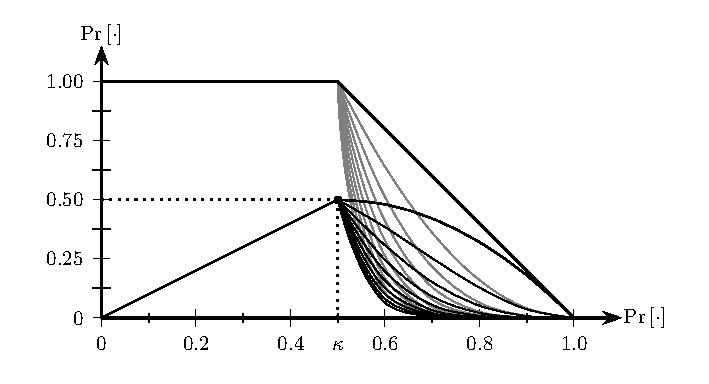
\includegraphics[scale=0.85]{figures/1102-simulation-failure-ii}
   \caption{Knowledge-extraction failure as function of verification success. The $x$-axis corresponds to the verification success and $y$-axis corresponds to the failure probability. The upper collection of graphs  corresponds to the knowledge extraction failure for $\ell\in\set{1,\ldots,10}$ and the upper collection of graphs lower graph corresponds to the simulation failure for $\ell\in\set{1,\ldots,10}$. The optimal configuration where $\ell=1$ is drawn in bold. By increasing the value of $\ell$, the simulation failure drops faster when $\varepsilon>\kappa$ but this does not reduce the worst-case bound on the simulation failure.}
   \label{fig:knowledge-extraction-trade-offs}
\end{figure}

\paragraph{Round-efficient solution.}
More efficient way to reduce the knowledge error is to run several protocols in parallel. The latter does not change the soundness of the protocol, since the latter depends on witness indistinguishability that is preserved under parallel composition. It is also straightforward to see that the knowledge error indeed drops $2^{-k}$. There are $2^k$ potential challenges and if the verifier is able to answer at least two of them correctly, then at least two sub-protocol runs are successful with different challenges and we can extract the witness. In brief, the knowledge extractor has to find two successful verification runs in order to extract the secret. As the simulation is already successful, it is enough to use random challenges in order to reveal the second successful verification run with the same randomness. 

If we probe the verifier with random challenges, the probability that we get a successful run that is different from the one revealed in simulation is $(\varepsilon-\kappa)$ where $\varepsilon$ is the unknown success probability  for verification. Thus, the probability of continuos stream of failures after $\ell$ tries is 
\begin{align*}
\pr{\KEXTR^{\VVV}(\phi,\kappa)=\bot}
=
\begin{cases}
1,&\text{if }\varepsilon\leq\kappa\enspace,\\
(1+\kappa-\varepsilon)^\ell &\text{if }\varepsilon>\kappa\enspace.
\end{cases}
\end{align*}      
Hence, the probability of simulation failure if
\begin{align*}
\pr{\SFAIL}
=
\begin{cases}
\varepsilon,&\text{if }\varepsilon\leq\kappa\enspace,\\
\varepsilon(1+\kappa-\varepsilon)^\ell &\text{if }\varepsilon>\kappa\enspace.
\end{cases}
\end{align*}      
Figure~\ref{fig:knowledge-extraction-trade-offs-ii} shows that this setting offers different tradeoffs in terms of rewindings.	


\begin{figure}[!h]
   \centering
   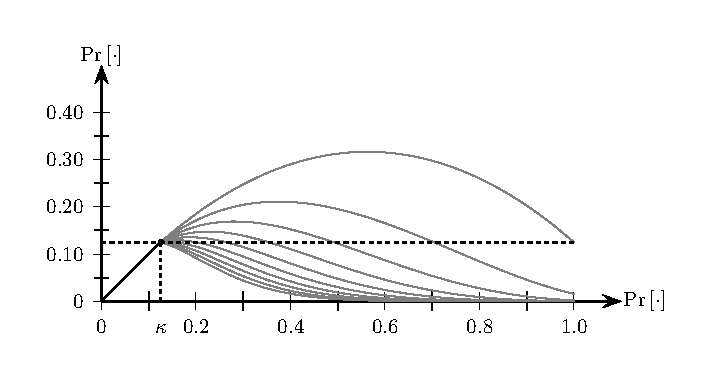
\includegraphics[scale=0.85]{figures/1102-simulation-failure-iii}
   \caption{Simulation failure as function of verification success when $\kappa=\frac{1}{8}$. The $x$-axis corresponds to the verification success and $y$-axis corresponds to the the simulation failure probability. The collection of graphs corresponds to $\ell\in\set{1,\ldots,10}$. The choice of the optimal value of $\ell$ is not a clear cut. The maximal value for simulation failure is above $\frac{1}{8}$ when $\ell\in\set{1,\ldots,9}$ but there is no rational reasons why the number of rewindings should be large enough to guarantee that the simulaten failure is equal to $\kappa$.}
   \label{fig:knowledge-extraction-trade-offs-ii}
\end{figure}
 
To find the maximal value on the simulation failure profile note that logarithm is a monotone function and thus we can minimise $\LLL=\log\pr{\SFAIL}$ instead. It is straightforward to see that 
\begin{align*}
\frac{\partial\LLL}{\partial\varepsilon}=\frac{1+\kappa-\varepsilon(\ell+1)}{\varepsilon(1+\kappa-\varepsilon)}\qquad \text{for}\qquad \varepsilon \geq\kappa
\end{align*}   
and thus the function is bound to have a single maximum in the location 
\begin{align*}
\varepsilon_*=\frac{1+\kappa}{1+\ell}
\end{align*}
father which the function starts to decrease. Consequently, if the number of rewindings \begin{align*}
\ell\geq \frac{1}{\kappa}\enspace,
\end{align*} 
the simulation failure is quarantined to decrease after $\varepsilon\geq \kappa$ and simulation failure coincides with knowledge error. For other choices of $\ell$ the maximal simulation failure is 
\begin{align*}
p_*=\max_{\varepsilon\in[0,1]}\pr{\SFAIL}
=\frac{(1+\kappa)^{\ell+1}}{2+\ell}\cdot\Bigl(1+\frac{1}{\ell+1}\Bigr)^{\ell+1}\approx \frac{(1+\kappa)^{\ell+1}}{2+\ell}\cdot e
\end{align*}
To illustrate the asymptotic behaviour in the process $\kappa\to 0$, we can try different ways to increase $\ell$. By choosing $\ell=\Theta(\frac{1}{\kappa})$ we get
\begin{align*}
p_*\approx\frac{(1+\kappa)^{\frac{1}{c\kappa}+1}}{2+\frac{1}{c\kappa}}\cdot e\approx
e^{1+\frac{1}{c}}\cdot\frac{(1+\kappa)c\kappa}{2c\kappa+1}\approx \alpha\kappa\enspace.
\end{align*}  
In other words, if $\ell=\Theta(\frac{1}{\kappa})$ then the simulation failure is of order $\Theta(\kappa)$. The latter is not very good for getting tight simulation bounds. In order to get statistical difference $2^{-80}$ we have to do around $2^{80}$ rewindings, which makes the simulator $2^{80}$ times slower than the original attack code. 

The simulation failure does not have be of same order as the knowledge error $\kappa$. As the knowledge error decreases exponentially in terms of the protocol efficiency, we could in principle allow different tradeoffs between $p_*, \kappa, \ell$. Ideally, we would like that $p_*$ would decrease exponentially wrt $\ell$. As the second term in the approximation
\begin{align*}
\log p_*\approx 1-\log (2+\ell)+(\ell+1)\log(1+\kappa)\approx 1-\log (2+\ell)+(\ell+1)\kappa 
\end{align*}
cannot be of order $\ell$, the exponential decay of simulation failure is impossible. In fact the simulation failure can decrease as a function of $\ell$ only if 
\begin{align*}
\kappa\leq \frac{\log(2+\ell)}{\ell+1}\enspace.
\end{align*}      
Note that even if the third term remains constant and does not grow, the simulation failure  decreases at most linearly in $\log(\ell)$ and thus for any choice of $\kappa$ the simulation failure is still $\Omega(\frac{1}{\ell})$. In that sense, inversely proportional slowdown cannot be escaped with conventional methods.     
\end{solution}
\end{document}

